\subsection{SVM Results}
A total number of 16 different configurations of the SVM algorithm were studied, combining the values of the four kernels mentioned in the methodology section \ref{methodology-svm-sec} (linear, rbf, polynomial and sigmoid) with four different values for the $C$ value. After training and testing all these configurations of the SVM algorithm in each dataset, a previous preselection of the best models based on the accuracy were done. A Friedman test was done in order to see if there was statistical significant difference between the accuracy of the models and the one with the highest accuracy was selected for each dataset (hepatitis and mushroom). 
\newline

The best model for each dataset was trained and tested with the reduced dataset obtained after applying the methods discribed in the section \ref{reduced-methods-sec}. Consecutively, another statistical analysis was carry on in order to show which reduced method offered a better performance. 

\subsubsection{Hepatitis}
\begin{figure}[t]
    \centering
    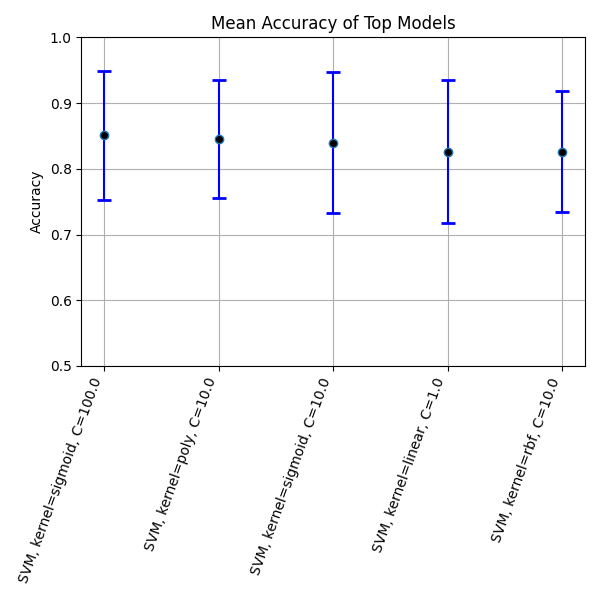
\includegraphics[width=\textwidth]{figures/svm/hepatitis/statistical_analysis_results.png}
    \caption{Mean accuracy for the five models of SVM with higher accuracies.}
    \label{fig:hep-svm-1}
\end{figure}


\begin{table}[h!]
\centering
\begin{tabular}{lccc}
\toprule
\textbf{Model} & \textbf{Accuracy} & \textbf{F1 Score} & \textbf{Time (s)} \\
\midrule
SVM, kernel=sigmoid, C=100.0 & 0.851 $\pm$ 0.010 & 0.91 $\pm$ 0.06 & 0.0006 $\pm$ 0.0005 \\
SVM, kernel=poly, C=10.0     & 0.84 $\pm$ 0.09 & 0.91 $\pm$ 0.05 & 0.0008 $\pm$ 0.0005 \\
SVM, kernel=sigmoid, C=10.0  & 0.84 $\pm$ 0.11 & 0.90 $\pm$ 0.07 & 0.0005 $\pm$ 0.0007 \\
SVM, kernel=linear, C=1.0    & 0.82 $\pm$ 0.11 & 0.89 $\pm$ 0.07 & 0.0011 $\pm$ 0.0006 \\
SVM, kernel=rbf, C=10.0      & 0.82 $\pm$ 0.09 & 0.89 $\pm$ 0.06 & 0.0011 $\pm$ 0.0006 \\
\bottomrule
\end{tabular}
\caption{Performance metrics for the best five SVM models with different kernels and regularization parameters.}
\label{tab:svm_metrics}
\end{table}

The Friedman test was performed obtaining a $p-value=0.4292$ that lead us to accept the null hypothesis that there are no significant differences between the five studied models. The model with higher mean accuracy in this case, according with the values shown on Table \ref{tab:svm_metrics} is the one with hyperparameters kernel=sigmoid and C=100.0, thus this one will be consider for the further analysis of the reduced datasets.



\subsubsection{Mushroom}
